\documentclass[]{article}

\usepackage[nottoc,numbib]{tocbibind}

\usepackage{amssymb,amsmath}
\setcounter{tocdepth}{3}
\usepackage{graphicx}
\usepackage{algorithm, algorithmic}
\usepackage{caption}
\usepackage{complexity}
\usepackage{subcaption}
\usepackage{tabularx}
\usepackage{cite}
\usepackage{pgfgantt}
\usepackage{listings}
\usepackage{xcolor}
\definecolor{darkgreen}{rgb}{0.0, 0.5, 0.0}
\graphicspath{{images/}}
\captionsetup{compatibility=false}
\lstset{
    language=Python,
    basicstyle=\ttfamily\small,
    keywordstyle=\color{blue},
    stringstyle=\color{red},
    commentstyle=\color{darkgreen},
    showstringspaces=false,
    numbers=left,
    numberstyle=\tiny\color{gray},
    breaklines=true,
    frame=single,
    captionpos=b,
    emph={__init__}, % list function keywords or names here
    emphstyle=\color{purple} % set your preferred function name color here
}

%\usepackage{setspace}
%%\singlespacing
%%\onehalfspacing
%\doublespacing

\DeclareMathOperator*{\argmax}{argmax}

\DeclareMathOperator*{\optimise}{optimise}
\DeclareMathOperator*{\subjectto}{subject\hspace{0.1cm}to}
%opening
\title{\textbf{AI-Driven Generative Design: Evolutionary Optimization of Residential Floor Plans}}
\author{Zuxing Wu, a1816653\\ \\Supervisor: Adel Nikfarjam\\ \\Master of Computer Science}

\begin{document}

\maketitle\nonumber

\newpage\nonumber

\tableofcontents

\newpage

% \begin{abstract}
% Abstract
% \end{abstract}

\section{Introduction}
\subsection{Aim}
Residential floor plan design is a complex and challenging task that requires careful consideration of various factors, such as room sizes, adjacencies, privacy, convenience, and orientations. Traditional methods of floor plan design are often time-consuming and labor-intensive, leading to suboptimal solutions. Evolutionary algorithms have been proposed as a promising alternative for optimizing floor plans, as they can efficiently explore the design space and generate high-quality solutions. This project aims to develop a new method for optimizing residential floor plans using evolutionary algorithms and address some limitations of previous research. The proposed method will involve the application of evolutionary algorithms to generate and evolve floor plans based on a novel representation scheme. The fitness of each floor plan will be evaluated based on several criteria (e.g.\ privacy, comfort, practicality, convenience). The performance of the proposed method will be evaluated using a set of benchmark problems and compared with existing approaches. The results of this project will contribute to the field of residential floor plan design and provide valuable insights into the application of evolutionary algorithms to architectural design problems.

\subsection{Motivation}
Residential floor plan design is a critical aspect of architectural design that involves the layout of rooms, corridors, and other spaces within a building. The design of a floor plan can have a significant impact on the functionality, convenience, comfort, ventilation and energy efficiency of a building. Traditional methods of floor plan design are often based on manual sketches or computer-aided design (CAD) tools, which can be time-consuming and labor-intensive. Moreover, these methods may not always produce optimal solutions, as they rely on the intuition and experience of the designer.

Evolutionary algorithms have been proposed as a promising alternative for optimizing floor plans, as they can efficiently explore the design space and generate high-quality solutions. Evolutionary algorithms are a class of optimization algorithms inspired by the process of natural selection. They work by maintaining a population of candidate solutions (individuals) and iteratively applying genetic operators (e.g.\ crossover, mutation) to generate new solutions. The fitness of each solution is evaluated based on a predefined fitness functions, which measure how well the solution satisfies the objectives of the optimization problems.

\section{Literature Review}
Previous research has explored the application of evolutionary algorithms to optimize residential floor plans. Brintrup et al.~\cite{10.1007/11732242_56} compared three interactive genetic algorithms (i.e., sequential IGA, multi-objective IGA, parallel IGA) on a multi-objective floor planning task, and found that the multi-objective IGA provides more diverse results and faster convergence for optimizing floor plans. They developed interactive evolutionary algorithms that allow designers to incorporate their preferences and constraints into the optimization process. This method has shown promising results in generating floor plans that meet both functional and aesthetic requirements.

It was found that proportional roulette wheel selection is the best parent selection method for the mating pool, and k-point crossover is the most effective for fitness evolutionary improvement~\cite{7844659}.
Combining evolutionary algorithms with greedy-like algorithms can help find near-optimal solutions in Automated Floor Plan Generation (AFPG), though it is a simplified model of multi-objective optimization by linear composition of the partial evaluation functions~\cite{doi:10.1177/1478077119832982}. Subramanian et al.~\cite{9675541} used a genetic algorithm with KD tree models in a web application to generate floor plans for even non-expert users.

Wang and Duan~\cite{WANG2023100238} tried to optimize floor plan design by focusing on energy consumption and consumer satisfaction, proving that the preferences of different types of consumers differed significantly. Therefore, different evaluation criteria are needed for satisfying different family types~\cite{WANG2023100238}. The quality and efficiency of residential floor plan design can be improved by combining Monte Carlo tree search algorithm (MCTS) and particle swarm optimization (PSO)~\cite{YAN2024110546}. The MCTS algorithm takes human experience into consideration so that it can compress the search space and improve the efficiency of the search process~\cite{YAN2024110546}. The PSO algorithm can handle continuous variables and is suitable for optimizing the size of rooms due to parallel processing~\cite{YAN2024110546}.

Enengy consumption, probable uniformity (PU), and spatial useful daylight illuminance (sUDI) are three objectives that are considered in the optimization process using NSGA-II algorithm, and the results show that the NSGA-II algorithm can provide a set of more sustainable floor plans that requires less computational power and time~\cite{CHAICHI2024108842}. Reliable metrics for evaluating the amount of light and the uniformity of light are tested in the optimization process, and can avoid unwanted convergence because they restrict each other~\cite{CHAICHI2024108842}.

Furthermore, the integration of machine learning techniques with evolutionary algorithms has gained attention in recent decades. For example, Wang et al.~\cite{WANG20051329} proposed a hybrid approach that combines a genetic algorithm with a neural network to predict the fitness of candidate solutions. This method significantly reduces the computational cost of evaluating large populations and accelerates the optimization process.

Overall, the literature indicates that evolutionary algorithms, particularly when combined with other optimization techniques and machine learning methods, offer a powerful tool for optimizing residential floor plans. These approaches not only improve the efficiency and quality of the designs but also provide flexibility in accommodating various design preferences and constraints.

\section{Methodology}
The methodology of this project involves the application of evolutionary algorithms to optimize residential floor plans. The process will be divided into several key stages: initialization of the population, representation of the floor plan, design of the evolutionary optimization framework, and performance evaluation. These stages are outlined below.

\subsection{Population Initialization}
The first step in the evolutionary process is to generate an initial population of residential floor plans. An efficient initialization strategy will be employed to ensure diversity within the population while adhering to basic architectural constraints, such as room adjacency and size. Specifically, the initialization process will involve generating a set of random rooms and arranging them into a floor plan layout. The rooms will be assigned random sizes and positions within the layout, with constraints on room adjacencies and widths. The initialization strategy will be designed to produce a diverse set of floor plans that can serve as a starting point for the evolutionary optimization process.

\subsection{Representation of Floor Plans}
Residential floor plans will be represented using a Python class, that encodes the spatial information of rooms, such as adjacency and dimension. This representation will be designed to allow for easy manipulation by evolutionary operators (e.g.~crossover or mutation) while preserving architectural feasibility and obeying relevant constraints. Most importantly, the representation will be flexible enough to accommodate different types of rooms, such as bedrooms, living rooms, kitchens, and bathrooms. The representation will also include the presence of doors and windows, and other architectural features. This representation will be used throughout the optimization process to encode, decode, and evaluate floor plans.

\subsection{Evolutionary Optimization Framework}
The evolutionary optimization framework currently will be based on particle swarm optmization (PSO) algorithm, which is suitable for optimizing the size of rooms due to parallel processing~\cite{YAN2024110546}. The PSO algorithm will be used to evolve the population of floor plans over multiple generations. The framework will involve the application of genetic operators, such as crossover and mutation, to generate new floor plans from the existing population. The fitness of each floor plan will be evaluated based on 4 types of criteria (e.g.\ privacy, comfort, practicality, convenience). The optimization process will be repeated for a specified number of generations or until a termination criterion is met.

If possible, more than one evolutionary algorithms will be used in the process of optimizing the floor plan. For example, Monte Carlo tree search algorithm (MCTS) handles discrete variables (e.g.\ room position) and particle swarm optmization (PSO) deals with continuous variables~\cite{YAN2024110546}.

\subsection{Fitness Function Design}
The fitness function will evaluate each floor plan based on several criteria:
privacy, comfort, practicality, convenience.
These criteria can be evaluated by a group of human evaluators, shown as Table~\ref{table1}.
\begin{table}[h]
    \centering
    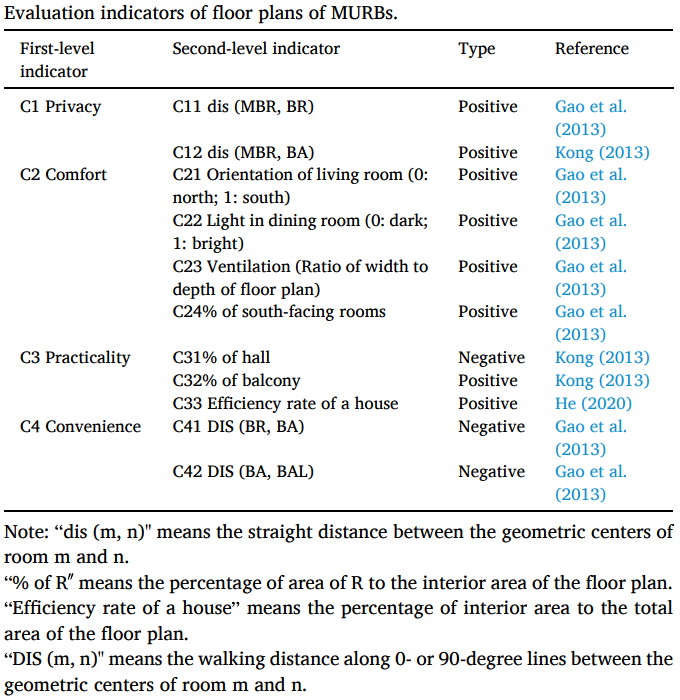
\includegraphics[width=0.8\textwidth]{image1.png}
    \caption{Evaluation indicators. Table 2 of Wang and Duan\cite{WANG2023100238}}\label{table1}
\end{table}

The straight distance between the geometric centers of room $m$ and $n$ is defined as:
\begin{equation*}
    \text{dis}(m, n) = \sqrt{(x_m - x_n)^2 + (y_m - y_n)^2}
\end{equation*}

The percentage of area of $R$ to the interior area of the floor plan is defined as:
\begin{equation*}
    \% \text{ of } R = \left( \frac{\text{Area of } R}{\text{Interior Area of Floor Plan}} \right) \times 100\%
\end{equation*}

The efficiency rate of a house is defined as the percentage of interior area to the total area of the floor plan:
\begin{equation*}
    \text{Efficiency Rate} = \left( \frac{\text{Interior Area}}{\text{Total Area}} \right) \times 100\%
\end{equation*}
The walking distance along 0- or 90-degree lines between the geometric centers of room $m$ and $n$ is defined as:
\begin{equation*}
    \text{DIS}_{\text{door}}(m, n) = \text{DIS}(m, \text{door}_m) + \text{DIS}(\text{door}_m, \text{door}_n) + \text{DIS}(\text{door}_n, n)
\end{equation*}


The proposed method will be implemented in Python. The optimization process will be carried out in two stages: initialization and mutation. The initialization stage will involve generating an initial population of floor plans using a novel strategy. The mutation stage will consist of iteratively applying genetic operators to the population to produce new generations. The fitness of each individual will be evaluated using multiple fitness functions that considers various factors such as the position of rooms, room sizes, and room adjacencies. The optimization process will be repeated for a specified number of generations or until a termination condition is met. The performance of the proposed method will be evaluated using a set of benchmark problems and compared with existing approaches.


\section{Plan vs Progress}
\subsection{Research Plan}
My research plan consists of four main phases at the beginning:
\begin{itemize}
    \item Phase 1
          \begin{enumerate}
              \item Population initialization
              \item Solution representation
          \end{enumerate}
    \item Phase 2
          \begin{enumerate}
              \item Evolutionary optimization
              \item Solution evaluation
          \end{enumerate}
\end{itemize}
Each phase involves specific tasks and activities that will be carried out over a period of 6 months. The timeline for the research plan is shown in the Gantt chart below. \\
\begin{ganttchart}[
        hgrid,
        vgrid,
        x unit = 1.4cm,
        y unit chart=0.7cm,
        title/.append style={fill=none},
        title label font=\bfseries\footnotesize,
        title label anchor/.append style={below=-1.6ex},
        include title in canvas=false,
        bar label font=\normalsize\scshape,
        bar label node/.append style={left=2ex},
        bar/.append style={fill=yellow!60},
        group/.append style={fill=cyan!80},
        bar incomplete/.append style={fill=red!30},
        progress label text={},
        group right shift=0,
        group top shift=0.7,
        group height=.3
    ]{1}{6}
    \gantttitle{2024.09--2025.02}{6} \\
    \gantttitlelist{9,10,11,12,1,2}{1} \\
    \ganttgroup{Phase 1}{1}{3} \\
    \ganttbar{Initialization}{1}{2} \\
    \ganttbar{Representation}{2}{3} \\
    \ganttgroup{Phase 2}{4}{6} \\
    \ganttbar{Optimization}{4}{5} \\
    \ganttbar{Evaluation}{5}{6}
    \gantttitle{Original Research Plan Timeline}{6} \\
\end{ganttchart}

However, the research plan has been adjusted according to the progress of the research. My supervisor and I both agree that the research plan should be adjusted to focus on the solution representation and solution evaluation first, and then move on to the evolutionary optimization and population initialization. The new research plan is shown in the Gantt chart below. \\
\begin{ganttchart}[
        hgrid,
        vgrid,
        x unit = 1.4cm,
        y unit chart=0.7cm,
        title/.append style={fill=none},
        title label font=\bfseries\footnotesize,
        title label anchor/.append style={below=-1.6ex},
        include title in canvas=false,
        bar label font=\normalsize\scshape,
        bar label node/.append style={left=2ex},
        bar/.append style={fill=yellow!60},
        group/.append style={fill=cyan!80},
        bar incomplete/.append style={fill=red!30},
        progress label text={},
        group right shift=0,
        group top shift=0.7,
        group height=.3
    ]{1}{6}
    \gantttitle{2024.09--2025.02}{6} \\
    \gantttitlelist{9,10,11,12,1,2}{1} \\
    \ganttgroup{Phase 1}{1}{3} \\
    \ganttbar[bar/.append style={fill=green!60}]{Representation}{1}{2} \\
    \ganttbar[bar/.append style={fill=green!60}]{Evaluation}{2}{3} \\
    \ganttgroup{Phase 2}{4}{6} \\
    \ganttbar{Optimization}{4}{5} \\
    \ganttbar{Initialization}{5}{6}
    \gantttitle{Current Research Plan Timeline}{6} \\
\end{ganttchart}


\subsection{Progress}
It can be seen from the Gantt chart above that the research plan has been adjusted to focus on the solution representation and solution evaluation first, and then move on to the evolutionary optimization and population initialization. It makes sense to focus on the solution representation and solution evaluation first, as solution representation is the prerequisite of solution evaluation, and the solution evaluation is the key to the success of the research. The evolutionary optimization and population initialization can be adjusted according to the progress of the research.

From the start of the project, I have completed the following tasks: 1. Solution representation, 2. Most of the solution evaluation functions. The solution representation is based on the Python class, which encodes the spatial information of rooms, such as vertexes, doors, windows, and adjacent rooms.
The solution evaluation is based on the evaluation indicators shown in Table~\ref{table1}. The fitness function is designed to assess each floor plan based on several criteria: privacy, comfort, practicality, and convenience. It includes 11 evaluation indicators from Wang et al.~\cite{WANG2023100238} research and 1 self-made indicator that are used to calculate the fitness of each floor plan.

All fitness values calculated from these indicators are normalized to the range of [0, 1] and then combined to form the final fitness value. The Min-Max normalization method is used to normalize the fitness values. The Min-Max normalization equation is defined as:
\begin{equation*}
    X_{\text{normalized}} = \frac{X - X_{\text{min}}}{X_{\text{max}} - X_{\text{min}}}
\end{equation*}
where $X$ is the original value, $X_{\text{min}}$ and $X_{\text{max}}$ are the minimum and maximum values of the evaluation indicator, respectively.

\section{Experimental Results}


\section{Conclusion}
In this project, Particle Swarm Optimization (PSO) is applied to the entire evolutionary optimization process for floor plan design. This approach is aimed at developing an efficient, user-friendly workflow that optimizes spatial layouts while meeting functional and aesthetic requirements. With PSO as the foundation, the goal is to complete the floor plan optimization process by implementing an adaptive, automated pipeline capable of producing high-quality layouts that align with user needs.

To ensure a smooth workflow, each component of the system will be tested rigorously for both efficiency and usability. Initial testing will focus on the system’s ability to generate optimized layouts within a feasible time frame. Any bottlenecks identified during testing will prompt optimizations to increase processing speed, ensuring the final system performs efficiently in a real-world setting. This will involve streamlining the PSO configuration and refining the interaction between components, as well as incorporating caching or faster algorithms where necessary to handle larger floor plans.

One additional aspect of this project is to generate vivid, detailed floor plans, including features such as furniture placement, texture suggestions, and enhanced visualizations to assist both designers and end-users in better understanding and interacting with the layouts. By incorporating these visual elements, the system aims to produce floor plans that are both functionally optimized and visually appealing, which can be valuable for designers as well as clients.

Moreover, the project will explore integration with AI models to further enhance the system’s capabilities. By using AI, the floor plan generation process can be augmented to suggest or adapt layouts based on user preferences or trends in design, making it a more versatile tool for various applications. This integration would also involve machine learning techniques that learn from user feedback to iteratively improve the generated layouts, aligning them more closely with client needs over time.

\section{Plagiarism Declaration}
I hereby declare that this submission is my own work and to the best of my knowledge, it contains no material previously published or written by another person, except where due to acknowledgment is made. Furthermore, I believe that it contains no material which has been accepted for the award of other degree or diploma in any university or other tertiary institutions.


\bibliographystyle{abbrv}
\bibliography{MyReferences}

\end{document}

